\subsection*{Establecimiento}
\addcontentsline{toc}{subsection}{Establecimiento}

En el siguiente apartado se describen los costos e inversiones necesarios para la creación de la empresa, teniendo en cuenta las inversiones requeridas para el diseño, desarrollo y despliegue del software. Con base en lo anterior, se requieren recursos económicos, humanos, administrativos y preoperativos, los cuales serán descritos a continuación:

\subsubsection*{Activos fijos tangibles}
\addcontentsline{toc}{subsubsection}{Activos fijos tangibles}

Los activos fijos tangibles se dividen en los múltiples dispositivos que van a hacer parte del área operacional y administrativa. Siendo fundamentales para dar inicio al proyecto. A continuación, se detallan en la tabla \ref{TablaActivosTangibles}:

\begin{table}[H]
	\centering
	\caption[{Activos tangibles}]{\centering Tabla de activos tangibles. \textit{Fuente:} Autores.}
	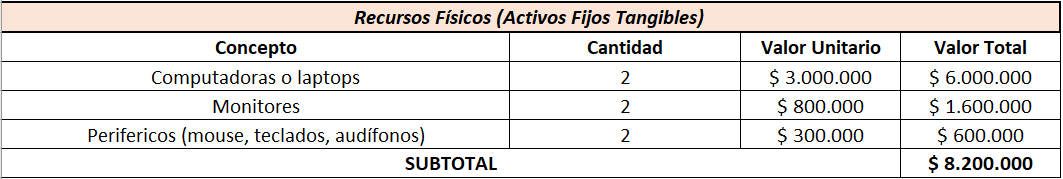
\includegraphics[width=13cm]{Imagenes/ActivosTangibles.png}
	\label{TablaActivosTangibles}
\end{table}

\subsubsection*{Activos fijos intangibles}
\addcontentsline{toc}{subsubsection}{Activos fijos intangibles}

Los activos fijos intangibles corresponden a los procesos financieros y legales que una empresa debe tener en cuenta para su constitución y funcionamiento. Estos se describen en la tabla \ref{TablaActivosIntangibles}.

\begin{table}[H]
	\centering
	\caption[{Activos tangibles}]{\centering Tabla de activos intangibles. \textit{Fuente:} Autores.}
	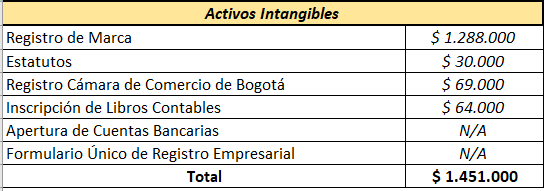
\includegraphics[width=12cm]{Imagenes/ActivosIntangibles.png}
	\label{TablaActivosIntangibles}
\end{table}

\subsubsection*{Total activos fijos}
\addcontentsline{toc}{subsubsection}{Activos fijos intangibles}

En la tabla \ref{TablaActivosFijos} se presenta un resumen del total de la inversión necesaria para la adquisición de los activos fijos, así como el capital de trabajo requerido para llevar a cabo el proyecto.

\begin{table}[H]
	\centering
	\caption[{Activos fijos}]{\centering Tabla de activos fijos. \textit{Fuente:} Autores.}
	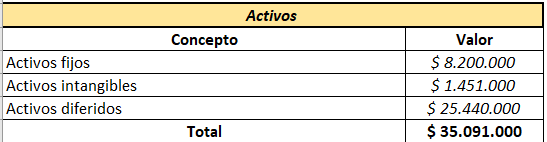
\includegraphics[width=12cm]{Imagenes/ActivosFijos.png}
	\label{TablaActivosFijos}
\end{table}

\subsubsection*{Financiamiento}
\addcontentsline{toc}{subsubsection}{Financiamiento}

En la tabla \ref{TablaFinanciamiento} se muestra la inversión necesaria para la fase inicial del proyecto, la cual debe evaluarse considerando tanto el aporte social (dado por los integrantes del proyecto) como el financiamiento proveniente de una entidad bancaria.

\begin{table}[H]
	\centering
	\caption[{Tabla de financiamiento}]{\centering Tabla de financiamiento. \textit{Fuente:} Autores.}
	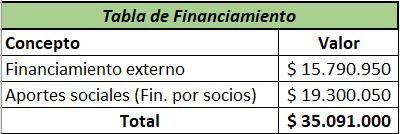
\includegraphics[width=11cm]{Imagenes/TablaFinanciamiento.png}
	\label{TablaFinanciamiento}
\end{table}


